% !TEX root = ../../main.tex
% !TeX spellcheck = de_DE

\chapter{Stand der Technik}
Dieses Kapitel behandelt den Forschungsstand.
Dazu gehören neuronale Netze, GANs inklusive zugehöriger Fachbegriffe, Namen und Methodiken.
Außerdem werden verschiedene Frameworks erläutert, die die Implementierung von Netzarchitekturen erleichtern.
Schließlich werden auch verwandte Arbeiten beleuchtet.

\section{Neuronale Netze}
Künstliche Neuronale Netze stellen ein Teilgebiet des Bereichs Künstliche Intelligenz dar.
Durch sie können komplexe Aufgaben, wie Gesichtserkennung, Erkennung von Betrugsfällen oder die Generierung von Bildern mit Computerprogrammen gelöst werden.
In der folgenden Abbildung ist eine Beispielarchitektur visualisiert:

\begin{figure}[H]
	\centering
	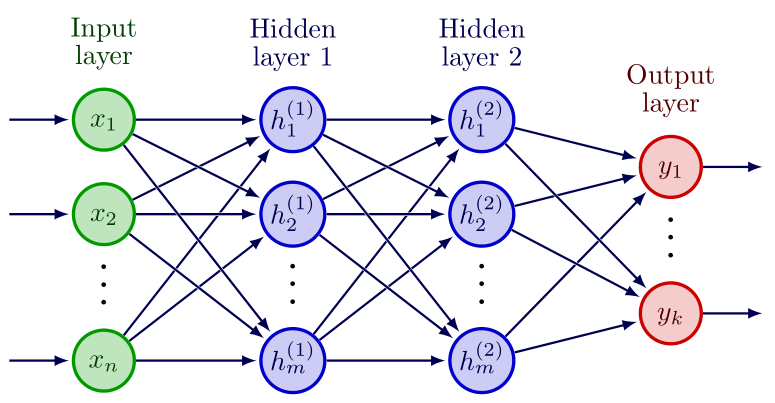
\includegraphics[width=12cm]{kapitel/2_stand_der_technik/img/neural-network.png}
	\caption[Darstellung eines Neuronalen Netzes]{Darstellung eines Neuronalen Netzes.}
	\label{img:neural-networks}
\end{figure}

Neuronale Netze bestehen aus synthetischen Neuronen, wobei sich beides am jeweiligen biologischen Vorbild orientiert.
In der Grafik \cref{img:neural-networks} sind die Neuronen als farbige Kreise gekennzeichnet.
Die Aufgabe eines Neurons besteht in der Umwandlung eines oder mehrere Eingangssignale in ein Ausgangssignal.
Für die Umwandlung wird beispielsweise die Summe aller Eingaben berechnet, auf eine Aktivierungsfunktion angewendet und an alle Ausgaben weitergegeben.
\newline

Neuronen sind in der Regel in Schichten sortiert, die jeweils mit der vorherigen Schicht verbunden sind.
Damit die Neuronen der verschiedenen Schichten miteinander kommunizieren können, gibt es Übergänge, die in \cref{img:neural-networks} als schwarze Linien dargestellt sind.
Jeder Übergang besitzt ein Gewicht, das mit dem zu übertragenden Wert multipliziert wird.
So wird die Komplexität des Modells erhöht, wodurch schwierigere Aufgaben gelöst werden können.
\newline

Die Berechnung des Ausgabewertes wird durch die folgende Formel mit dem Ausgabewert $y$, Eingaben $x$, Gewichte für die jeweiligen Eingaben $w$ und Aktivierungsfunktion $\varphi$ verdeutlicht:

\begin{equation}
	y = \varphi ( \sum_{n=0}^N x_n * w_n).
\end{equation}

\subsection{Training}
Neuronale Netze werden nicht im klassischen Sinne programmiert, stattdessen werden definierte Netzarchitekturen trainiert.
Der Trainingsprozess orientiert sich hierbei wieder an natürlichen Lernvorgängen.
Dazu gehören unter anderem Supervised- und Unsupervised-Learning.
Der Unterschied zwischen den Verfahren liegt in der Existenz eines vorgegebenen Erwartungswertes für jede Eingabe.
Beide Verfahren haben Vor- und Nachteile, ihre Anwendung ergibt sich in der Regel aus den vorliegenden Daten und gewünschten Ergebnissen.

Ziel des Trainings ist die Anpassung der Weights, der Übergänge zwischen den Neuronen.
Sie werden im Kontext des Trainingsprozesses auch Parameter genannt.
Durch die Anpassung der Parameter passt sich das Netz den Daten an und erlaubt so verschiedenste Aufgaben zu lösen.
So können dann beispielsweise Gesichter in Bildern oder Betrugsfälle in Abbuchungen erkannt werden.
\newline

Für das Training müssen zusätzliche Konfigurationen festgelegt werden, die Hyperparameter genannt werden.
Im Gegensatz zu den Parametern neuronaler Netze werden sie durch das Training nicht verändert.
Bei Hyperparametern handelt es sich zum Beispiel um die Anzahl an Neuronen in einer bestimmten Schicht \cite{hyperparameters-gan-using-genetic-algorithm}.
Die Auswahl an Hyperparametern hat einen sehr großen Einfluss auf den Trainingserfolg von Modellen.
Zusätzlich unterscheiden sich optimale Hyperparameter je nach Architektur und zugrundelegenden Daten, weswegen eine eigene Hyperparametersuche immer sinnvoll ist. \todo{quelle}
Es sind auch nicht alle Hyperparameter gleichbedeutend für den Trainingserfolg, beispielsweise die Lernrate hat einen besonders großen Einfluss auf den Trainingserfolg \cite{learning-rate-most-important}.
Die Suche nach optimalen Hyperparametern ist sehr komplex, weswegen spezielle Suchverfahren entwickelt wurden. \todo{Überleitung zu Hyperparam Suchverfahren?}

\subsection{Verschiedene Schichten}
Wie bereits erwähnt, werden Neuronale Netze mittels Schichten aufgebaut.
Es existieren verschiedene Typen von Schichten, welche jeweils ganz bestimmte Aufgaben übernehmen.
Die wichtigsten Arten sollen in der folgenden Aufzählung kurz erläutert werden.

\subsubsection{InputLayer und OutputLayer}
Diese beiden Schichten gehören nicht zu der Blackbox, die ein Neuronales Netz charakterisiert.
Wie man bereits in der Abbildung \ref{img:neural-networks} erkennen konnte, werden über diese beiden Schichten mit dem Modell interagiert.
Das InputLayer definiert, welche Formfaktor die zu verarbeiteten Daten haben müssen.
Diese Daten sind immer in der Form eines Tensors gegeben und können sich über mehrere Dimensionen spannen. 
So repräsentiert die Formangabe \textit{[3, 50]} eine Matrix mit drei Reihen und 50 Spalten.
Diese Formangabe spielt auch bei anderen Schichten innerhalb des Neuronalen Netzes eine Rolle.
So hat jede einzelne Schicht eine Input- und Output-Größe.
\newline

Das OutputLayer ist normalerweise keine spezielle, dedizierte Schicht.
In der Regel, repräsentiert die letzte im Modell angeschlossene Schicht die Ausgabe.

\subsubsection{DenseLayer}
Das DenseLayer ist eine so genanntes \textit{deeply connected Layer}.
Das bedeutet, dass jedes Neuron mit jedem Neuron der vorherigen Schicht verbunden ist.
Auch dies kann in der Abbildung \ref{img:neural-networks} beobachtet werden, wobei beide blauen Schichten diesem Typ entsprechen.
Diese Eigenschaft macht das DenseLayer zu einem der weitestverbreiteten Schichten innerhalb Neuronaler Netze \cite{dense-layer}.
Vor allem im Bereich der Klassifizierung wird es häufig eingesetzt.

\subsection{ConvolutionalLayer und ConvolutionalTransposeLayer}


\subsubsection{FlattenLayer und ReshapeLayer} 
\todo{das hier erklären?}

\subsubsection{ActivationLayer und BatchNormalization}
Aktivierungsfunktionen sind ein wichtiges Werkzeug innerhalb Neuronaler Netze.
Sie bilden ein großes Spektrum an Werten auf einen kleinen Bereich ab.
Beliebte Funktionen sind dabei LeakyReLU, Tanh oder Softmax.
Häufig kann man sie am Ende eines Modells finden.
Nicht selten stellen sie das OutputLayer eines Netzes dar.
Jedoch werden sie auch innerhalb der HiddenLayer verwendet.
Sie folgen häufig auf Dense oder ConvolutionalLayer.
\newline





\subsubsection{MultiplyLayer}
Diese Schicht repräsentiert, wie der Name vermuten lässt, einen arithmetischen Operator.
Es werden mehrere Input-Tensoren zu einem Output-Tensor multipliziert.
Dabei muss natürlich sichergestellt werden, das alle hineingegebene Tensoren den gleichen Formfaktor besitzen.
Diese Schicht wird eine große Rolle bei der Architekturen von GANs spielen, da dort zwei Inputs zu einem Output vereinigt werden müssen.

\section{General Adversarial Network}
Der Begriff \acrfull{GAN} ist auf Ian Goodfellow zurückzuführen \cite{gan-original-paper}.
Das Wort bezeichnet ein Konstrukt aus 2 neuronalen Netzen, die sich gegenseitig trainieren.
Durch das spezielle Training gelingt die Generierung von realistischen synthetischen Daten.
Solche Daten können dann zum Beispiel für das Training anderer neuronalen Netze \cite{gan-application-augmenting-training-data}, in der Bildverarbeitung \cite{gan-application-upscaling, gan-application-blending} und vielen weiteren Anwendungsgebieten verwendet werden \cite{gan-application-dna-optimizes-protein-functions, gan-application-audio-synthesis}.

\begin{figure}[H]
	\centering
	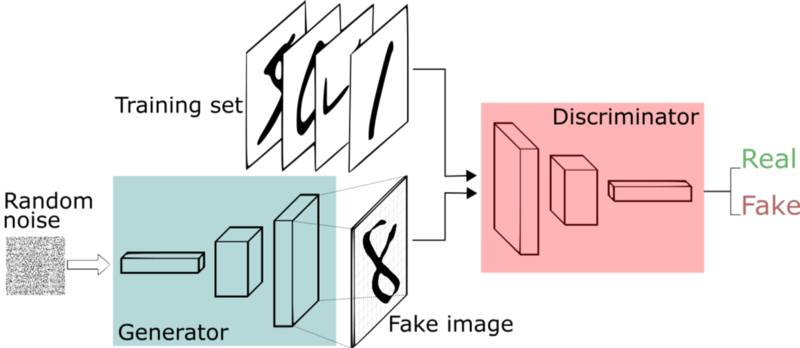
\includegraphics[width=12cm]{kapitel/2_stand_der_technik/img/GAN.png}
	\label{img:gan}
	\caption{Generative Adversarial Network (Bild von Thalles Silva \cite{img-gan})}
\end{figure}

Die beiden Netze eines \acrshort{GAN}s werden in den Generator und den Discriminator unterschieden.
Aufgabe des Generators ist die Generierung von synthetischen Daten.
Dafür wandelt er eine zufällige Eingabe in einen möglichst realistischen Output um.
Die zufällige Eingabe dient als Basis für die Ausgabedaten.
Das ist notwendig, da der Umwandlungsprozess selbst deterministisch ist, aber trotzdem eine Vielzahl an unterschiedlichen Daten generiert werden soll.
\newline

Der Output des Generators wird vom Discriminator klassifiziert.
Dafür wird er sowohl auf die generierten Daten als auch einen Bestand an echten Daten trainiert.
Sein Ziel ist es, die falschen Daten des Generators zu identifizieren.
Ziel des Generators hingegen ist es, den Discriminator zu täuschen und die generierten Daten als echt wirken zu lassen.
\newline

Ian Goodfellow bezeichnet den Lernprozess auch als Minimax-Spiel, bei dem die Ausgabe des Discriminators die zu optimierende Größe ist.
Das bedeutet, der Generator versucht die Genauigkeit des Discriminators zu verringern, während der Discriminator sie erhöhen möchte. \cite{gan-minimax}

\subsection{Ausprägungen von GANs}
In diesem Kapitel die Architekturmodelle CGAN, Dense-GAN und DC-GAN vorgestellt.
Das ist deshalb wichtig, da die zugehörigen Bezeichnungen in der Literatur nicht klar definiert sind.
So werden beispielsweise je nach Kontext der Arbeit sowohl Cycle-GANs als auch Conditional GANs als CGANs bezeichnet.

\subsubsection{CGAN}
\todo[inline, shadow]{verständlich?}
Das \acrfull{CGAN} \cite{mirza2014conditional, gan-conditional} erlaubt die Beeinflussung der Generierung durch Labels.
Dafür wird der normale Trainingsablauf eines GANs durch Labels erweitert, wie in der Abbildung dargestellt.
\begin{figure}[H]
	\centering
	% Dokument: https://drive.google.com/file/d/1qso4iFm3YGvxG3NmwlUdatspkJdja00B/view?usp=sharing
	% beim Export auf 300% Zoom stellen
	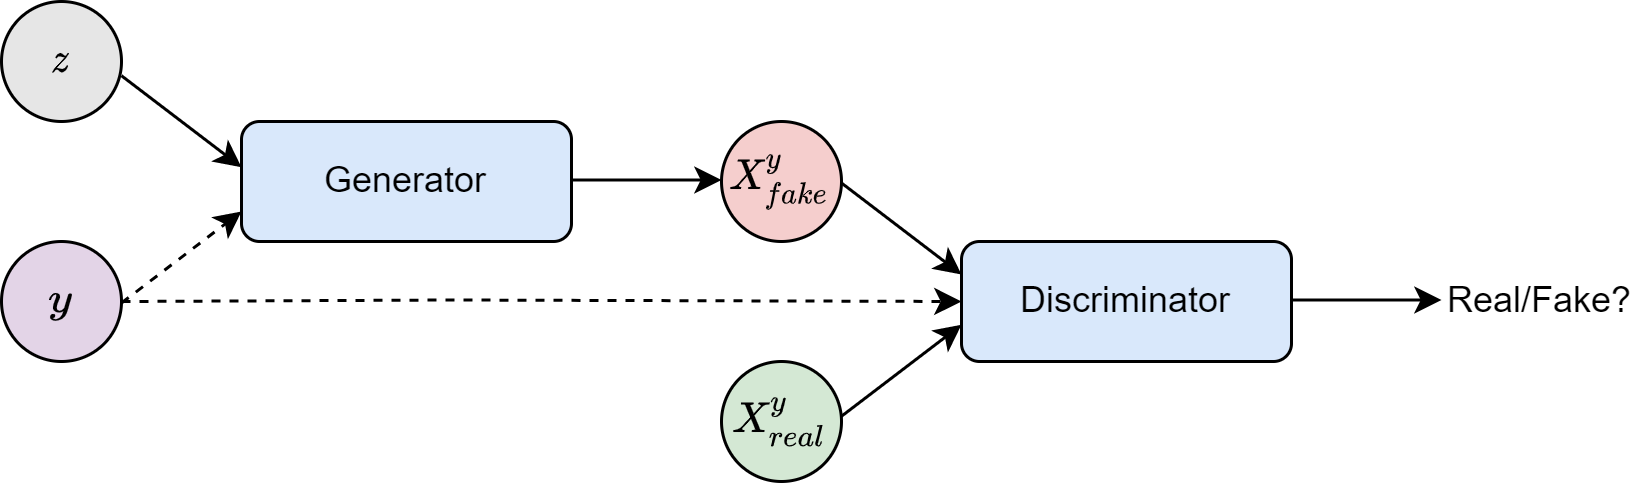
\includegraphics[width=14cm]{kapitel/2_stand_der_technik/img/cgan-vs-gan.drawio.png}
	\caption[Flowchart Trainingsprozess GAN und CGAN]{Flowchart Trainingsprozess GAN (nur durchgestrichene Pfeile) und CGAN (alle Pfeile)}
	\label{flowchart-cgan-vs-gan}
\end{figure}

Das Datenlabel $y$ wird sowohl für die Generierung der Bilder, als auch bei der Verifizierung durch den Discriminator genutzt.
Dafür erhalten sowohl Discriminator als auch Generator eine weitere Eingabe.
So kann der Discriminator den Zusammenhang zwischen Label und bestimmten Eigenschaften der Daten lernen.
Dadurch ist dann der Generator gezwungen, diese Eigenschaften zu berücksichtigen, um den Discriminator wieder zu täuschen.
\newline

Sobald das \acrshort{GAN} zufriedenstellend trainiert ist, können so labelspezifische Daten generiert werden.
Das kann in der Praxis sehr günstig sein, wenn zum Beispiel das Krankheitsbild einer bestimmten Krankheit generiert werden soll.
Die Nutzung des Conditional Discriminators erlaubt zusätzlich die Identifizierung einer bestimmten Krankheit auf einem Bild.

\subsubsection{Dense-GAN}
Eine Dense-GAN nutzt sowohl für Discriminator als auch für den Generator Dense Layer beziehungsweise Fully Connected Layer.
Dense Layer bestehen aus Neuronen, die jeweils mit jeder Ausgabe der vorherigen Schicht verknüpft sind.
\newline

Vorteil dieses Architekturmodells ist seine große Flexibilität.
Mithilfe der Dense Layer und einer ausreichend großen Architektur lassen sich theoretisch alle Zusammenhänge eines Datensets lernen.
\newline

Nachteil sind die vielen zu lernenden Parameter.
Pro Schicht ergeben sich $|weights| = inputs * outputs$, was bei größeren Architekturen einen erheblichen Lernaufwand bedeutet.
Insbesondere im Vergleich zu Convolutional Layern macht dies einen enormen Unterschied.

\subsubsection{DC-GAN}
\todo{Belege}
Ein DC-GAN oder auch Deep Convolutional GAN besteht hauptsächlich aus Convolutional Layern.
Im Generator finden vor allem Convolutional Transposed Layer ihre Anwendung.
Convolutional Transpose Layer funktionieren wie Convolutional Layer, jedoch vergrößern sie Ausschnitte, statt sie zu komprimieren.
Im Discriminator werden Convolutional Layer genutzt, um die Datenmenge auf eine Entscheidung klein zu skalieren.
Im letzten Schritt des Discriminators existiert in der Regel ein Dense Layer, um die finale Entscheidung zu berechnen.
\newline

Vorteil dieser Architektur sind die vergleichsweise wenigen zu lernenden Parameter.
Die geringe Anzahl an Parametern sind der Tatsache geschuldet, dass es pro Ausgabe-Dimension nur einen Filter für das Convolutional Layers gibt.
Dadurch ist auch die Parameteranzahl der Convolutional Layer unabhängig von der Bildgröße.

Zusätzlich zur geringen Parameteranzahl fördern die Filter auch das Verständnis von Zusammenhängen zwischen benachbarten Pixeln.
Die Zusammenhänge werden dabei implizit durch die Architektur vorgegeben und müssen nicht erst aufwändig gelernt werden.
\newline

Die Tatsache, dass die Filter der Convolutional Layer Zusammenhänge zwischen benachbarten Datenpunkten implizieren ist auch gleichzeitig ein Nachteil der Architektur.
Sollten die Beziehungen zwischen nahen Datenpunkten nicht existieren, können falsche Zusammenhänge vorausgesetzt werden, was zu schlechteren Ergebnissen führen kann.
Insgesamt ist eine solche Architektur somit nicht so flexibel wie eine Dense Architektur, aber dafür effizienter.

\section{Metriken}
\subsection{Accuracy}
\todo{falls in ergebnisse verwendet werden wird. evtl auch loss}
\subsection{FID}	
% TODO quelle: https://wandb.ai/ayush-thakur/gan-evaluation/reports/How-to-Evaluate-GANs-using-Frechet-Inception-Distance-FID---Vmlldzo0MTAxOTI
Die Bewertung von Trainingserfolgen durch GANs ist nicht trivial, denn für die Bewertung muss die Qualität der generierten Bilder eingeschätzt werden.
Erstmals in \cite{fid} wurde dafür der \acrfull{FID} aufgezeigt.

Für die Berechnung des \acrshort{FID} werden zunächst die Ausgaben eines Layers des Inception Nets von Trainingsdaten und generierte Daten gesammelt.
Danach wird aus den Werten der Embeddingschicht der Durchschnitt und die Kovarianz berechnet und verrechnet.
Die nachfolgende Formel \cite{are-gans-created-equally} zeigt die genaue Berechnung auf, wobei sich $x$ und $g$ auf die Trainingsdaten und genierten Daten beziehen

\begin{equation}
	\FID(x, g) = ||\mu_x - \mu_g||_2^2 + \Tr(\Sigma_x + \Sigma_g - 2(\Sigma_x \Sigma_g)^{\frac{1}{2}}).
\end{equation}

Die \acrshort{FID} erlaubt die Einschätzung der Qualität der Bilder korrelierend zu menschlichen Einschätzungen.
% TODO mode collapse erklären
Auch die Vielfalt wird bewertet, indem zum Beispiel Mode-Collaps als negativ bewertet wird und gleichzeitig eine relative Robustheit gegenüber Rauschen besteht (im Vergleich zum Inception Score \cite{are-gans-created-equally}). 

\begin{figure}[H]
	\centering
	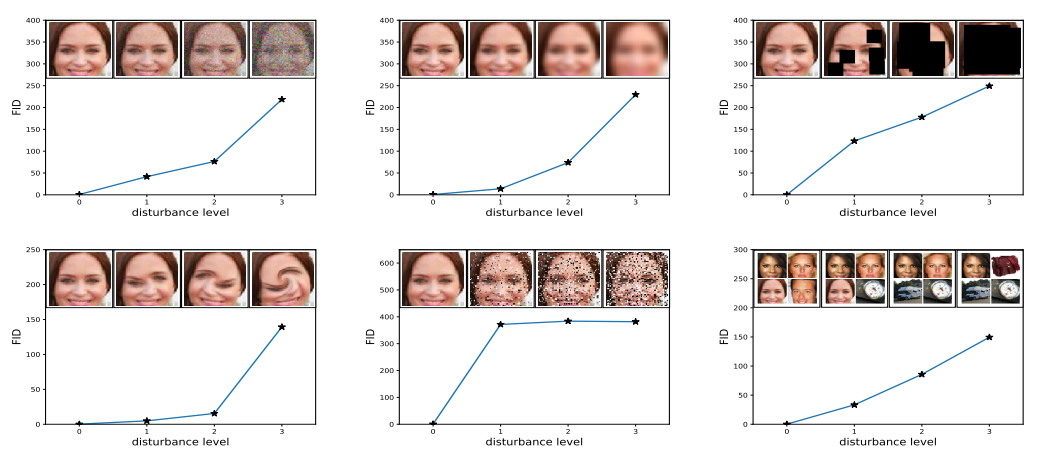
\includegraphics[width=16cm]{kapitel/2_stand_der_technik/img/fid-example.png}
	\caption[Beispiel von unterschiedlichen FID-Werten]{Beispiele unterschiedlicher FID-Werte aus \cite{fid}.\\ \textbf{Oben Links:} gaußsches Rauschen; \textbf{Oben Mitte:} gaußscher Weichzeichner; \textbf{Oben Rechts:} schwarze Rechtecke; \textbf{Unten Links:} verwirbelte Bilder; \textbf{Unten Mitte:} Salt and Pepper Noise; \textbf{Unten Rechts:} CelebA Datensatz mit ImageNet Bildern versetzt }
	\label{fid-example}
\end{figure}

\section{Hyperparameter}
\todo{was ist ein hyperparemter?}
\subsection{Auswahl an Hyperparametern}

\subsubsection{Learning-Rate}
Die Learning-Rate entspricht dem Faktor \(\alpha\), welcher die Intensität des Gradientenabstiegs bestimmt:  
\begin{equation}
	\theta  =  \theta  - \alpha   \nabla_{ \theta }  J( \theta ).
\end{equation}

\todo[]{mit quellen backen}
Bei zu großem \(\alpha\) kann der Trainings-Fehler anfangen zu oszillieren oder sogar größer werden.
Bei zu kleinem \(\alpha\) konvergiert der Fehler zu langsam oder bleibt in einem lokalen Minimum stehen. 
Es ist anzumerken, dass die oben gezeigt Formel dem einfachen Gradientenabstieg entspricht.
Normalerweise werden fortgeschrittenere Algorithmen angewendet, welche jedoch weiterhin auf dem Gradientenabstieg basieren.
So können weitere Parameter, wie das \textit{Momentum} die Abstiegsweite beeinflussen.
\newline

Für alle Architekturen wird der Adam-Optimierungs-Algorithmus angewendet.
\todo{warum? 1. bekannt / standart, 2. schnelle ergebnisse}
\todo{wie funktioniert er grob?}

\subsubsection{Batch-Size}
Ähnlich wie die Learning-Rate ist auch die Batch-Size ein sehr beliebter Hyperparameter und wird in unterschiedlichen Tutorials referenziert \cite{tutorial:tune-batch-size-analyticsvidhya, tutorial:tune-batch-size-machinelearningmastery}.
Die Batch-Size beschreibt, wie viele Traingsdaten verabeitet werden, um einen Gradientenabstieg der Gewichte durchzuführen.
Grundsätzlich führt eine kleine Batch-Size zu besseren Ergebnissen.
Ein Experiment über kleine Batch-Größen im Bezug auf Neuronale Netze kam zu folgenden Ergebnis: 

\begin{displayquote}
	\enquote{In all cases the best results have been obtained with batch sizes m = 32 or smaller, often as small as m = 2 or m = 4.}
	\cite[S. 16, Z. 5-7]{small-batch-size}
\end{displayquote}

Eine kleinere Batch-Size führt dazu, dass der Fehler speziellere Fälle abbilden kann und damit eine Generalisierung unterbunden wird \cite{tutorial:tune-batch-size-machinelearningmastery}.
Jedoch ergibt sich aus einer kleineren Batch-Size ein Leistungs-Problem: die Berechnung des Fehlerwerts und die anschließende Optimierung der Gewichte wird häufiger durchgeführt.
Das führt logischerweise zu einer längeren Trainingsdauer pro Epoche.

\subsubsection{Dropout}
Der Dropout definiert die Größe eines zufälligen Anteils an Neuronen, die dann inklusive ihrer Verbindungen im Training deaktiviert werden.
Das führt dazu, dass immer andere Neuronen das Ergebnis beeinflussen, was Overfitting entgegenwirkt \cite{JMLR:v15:srivastava14a}.
Bei Overfitting lernt das neuronale Netz Besonderheiten der Trainingsdaten, die aber in der Realität nicht vorkommen.
Dadurch erzielt es sehr gute Ergebnisse im Training, spätestens bei der Anwendung ist die Leistung jedoch verhältnismäßig schlecht.

% TODO https://machinelearningmastery.com/dropout-for-regularizing-deep-neural-networks/

\subsubsection{Smoothness - Onesided Label Smoothing}
Onesided Label Smoothing entstammt einer Idee von Ian Goodfellow \cite{ian-goodfellow-onesided-label-smoothing}.
Sie verändert den Loss, indem sie den Optimalwert für das gewünschte Ergebnis anpasst.
Dafür wird die optimale Ausgabe des Discriminators von 1 oder 0 auf beispielsweise 0.9 oder 0.1 gesetzt.
Der Prozess hilft besonders gegen Adversarial Examples.
Adversarial Examples sind sehr geringe Unterschiede in den Bildern, die die Klassifikation des Discriminators aber sehr stark beeinflussen.
Sollte der Generator diese Änderungen lernen, kann er den Discriminator täuschen, ohne dass sich die Bildqualität erhöht.

\begin{figure}[H]
	\centering
	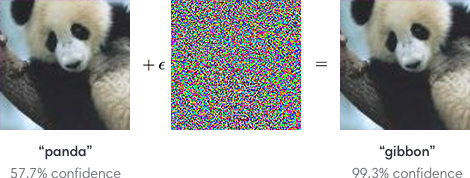
\includegraphics[width=10cm]{kapitel/2_stand_der_technik/img/adversrial-example.png}
	\caption[Adversarial Example]{Durch das (nicht sichtbare) zusammenführen der 2 Bilder, wird der Panda fälschlicherweise als Gibbon klassifiziert}
	\label{smoothness-adversarial-example}
\end{figure}

\todo{Smoothness durch Onesided Label Smoothing ersetzen oder erklären, dass beides das gleiche ist?}

\subsection{Verfahren zur Bestimmung von Hyperparametern}
\label{chapter:verfahren-bestimmung-hyperparameter}
\todo{Quelle \cite{hyperparameters-search}}

Die Bestimmung guter Hyperparameter ist im Rahmen der Arbeit von großer Bedeutung, da verschiedene Architekturen auf ihre Effektivität und Effizienz untersucht werden sollen.
Der Vergleich verschiedener Architekturen mit gleichen Hyperparametern ist hingegen nicht fair, da der Einfluss der Hyperparameter auf das Ergebnis so groß ist.
\newline

Für die Suche nach optimalen Hyperparametern gibt es verschieden Verfahren, die im Folgend vorgestellt werden.
Dabei wird sich auf die Grid Search, Random Search und den Genetic Algorithm beschränkt, da diese die beliebtesten Algorithmen zur Optimierung sind \cite{hyperparameters-search-comparison-focus-genetic}.
Die Verfahren werden zusätzlich mit der manuellen Suche verglichen, um eine allgemeinere Einschätzung gewährleisten zu können.

\subsubsection{Manuelle Suche}
Die manuelle Suche ist das simpelste vorgestellt Verfahren.
Hierfür werden nur die Hyperparameter vor jedem Training manuell festgelegt.
Nach einem Trainingsdurchlauf können dann die Ergebnisse analysiert, Hyperparameter angepasst und die verbesserte Version erneut trainiert werden.

%Die manuelle Suche ist vor allem bei unwichtigen Hyperparametern sinnvoll, da dort bekannte Standardwerte gesetzt werden können.
%Für eine gründliche Suche aller Hyperparameter ist die manuelle Suche allerdings viel zu aufwändig.

\subsubsection{Grid Search}
Bei der Grid Search \cite{hyperparameters-grid-search} werden zunächst die zu untersuchenden Hyperparameter ausgewählt.
Danach erfolgt die Definition eines Suchintervalls inklusive Intervallschritten für jeden Hyperparameter.
Schließlich wird das neuronale Netzwerk für jede Kombination der Hyperparameterwerte trainiert und die Ergebnisse der einzelnen Durchläufe festgehalten.
Die Trainingsdurchläufe können dabei parallel stattfinden.

Nach dem Training ist es dann möglich, die einzelnen Ergebnisse zu vergleichen.
Dabei können dann Schemata erkannt und Kombinationen aussortiert werden.
%Es ist dann möglich die erfolgversprechendsten Netze weiter zu trainieren, oder direkt eine zufriedenstellende Kombination auszuwählen.
\newline

Insgesamt ist Grid Search sehr simpel zu implementieren, aber auch sehr ressourcenaufwändig.
Der exakte Aufwand hängt dabei stark von der Anzahl der möglichen Kombinationen der Hyperparameterwerte ab.
Da die Anzahl der Kombinationen der Hyperparameter exponentiell \todo{begründen?} wächst, nimmt auch der Aufwand mit der Anzahl an Werten sehr stark zu.
Durch die Möglichkeit von Parallelisierung findet die Grid Search in der Regel bessere Parameter als die sequentielle manuelle Suche in der gleichen Zeit \cite{hyperparameters-random-search}.

\subsubsection{Random Search}
Die Random Search \cite{hyperparameters-random-search} funktioniert ähnlich wie die Grid Search, nur werden zufällige Werte statt einem festgelegten Werteraster erzeugt.
Die zufälligen Werte haben den Vorteil, dass es weniger Werte-Überlagerungen im Vergleich zur den Raster-Kombinationen gibt, wie in \cref{randomsearch-vs-gridsearch} dargestellt.
Deswegen kann die zufällige Suche bei gleich vielen Durchläufen ein größeres Spektrum an Ergebnissen abdecken.
Mittels \textit{Automatic Relevance Determination} \cite{automatic-relevance-determination} ist es dann möglich, den Einfluss und Wertebereich der einzelnen Hyperparameter darzustellen.

\begin{figure}[H]
	\centering
	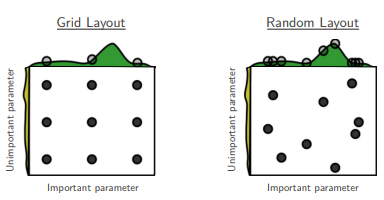
\includegraphics[width=10cm]{kapitel/2_stand_der_technik/img/random-vs-grid-search1.png}
	\caption[Vergleich zwischen Grid Search und Random Search]{
		Abbildung von 9 Optimierungsversuche der Funktion $f(x,y)=g(x)+h(x) \approx g(x)$.
		Über den Quadraten ist $g(x)$ und links $h(x)$ abgebildet.
		Während die Grid Search im Versuch nur 3 unterschiedliche Werte austestet, schafft die Random Search eine Suche über 9 verschiedene Punkte.
		\cite{hyperparameters-random-search}}
	\label{randomsearch-vs-gridsearch}
\end{figure}

Vorteil der Random Search im Vergleich zur Grid Search ist, dass keine Hyperparameter festgelegt werden müssen.
Das erlaubt eine unvoreingenommene Herangehensweise an die Suche.
\newline

Problem der Random Search ist vor allem, dass die Räume der guten Hyperparameter (\textit{Search Space}) sehr klein sind.
Dadurch ist nicht gewährleistet, dass ein zufälliger Wert auch den Raum der optimalen Werte trifft.
Jedoch erzielen Hyperparametersuchen mittels Random Search in der Regel trotzdem gute Ergebnisse.
Dem Grid Search Verfahren ist die Random Search allerdings nicht prinzipiell überlegen \cite{hyperparameters-random-search}.
\newline

Aufgrund ihrer Ähnlichkeit teilt sich die Random Search auch das Problem der Ressourcenintensivität mit der Grid Search.
Sobald ein sehr großes Spektrum an Hyperparametern untersucht werden soll, benötigt sie sehr viel Zeit.
Je nach zusätzlichen Optimierungen für die Wahl der Zufallswerte lässt sich die Random Search auch nicht unbedingt parallelisieren, was zu einer sehr langen Laufzeit führen kann.

\subsubsection{Genetic Algorithm}
Der Genetic Algorithm \cite{hyperparameters-genetic-algorithm} wandelt die Hyperparametersuche in einen evolutionären Entwicklungsprozess um.
Der Evolutionsaspekt des Algorithmus ist dabei eine Anlehnung an die natürliche Entwicklung in der Natur.
Diese Entwicklung zeichnet sich durch die Operatoren \textit{Selektion}, \textit{Kombination} und \textit{Mutation} aus, die der Algorithmus verwendet .
\newline

Für den Optimierungsprozess werden am Anfang mehrere zufällige Hyperparameterinstanzen erzeugt.
Die Instanzen werden dann trainiert und stehen im Wettbewerb um das beste Ergebnis.
Nach der Auswertung der Trainingsergebnisse werden die besten Instanzen selektiert und miteinander gekreuzt und oder mutiert.
\newline

Der Genetic Algorithm eignet sich besonders gut bei sehr vielen Hyperparametern.
Im Gegensatz zur Grid Search werden nicht immer alle Kombinationen ausprobiert, sondern nur einzelne, die sich bereits zuvor als vielversprechend herausgestellt haben.
Dadurch kann mit sehr großen Mengen an Hyperparametern umgegangen werden.
\newline

Allerdings ist der Genetic Algorithm vergleichsweise langsam, da die Evolutionsschritte sequentiell ablaufen müssen.
Erst bei einer hohen Anzahl an Hyperparametern oder einem sehr großen Suchraum ist der Genetic Algorithm effizienter als eine Grid Search \cite{hyperparameters-search-comparison-focus-genetic}.

\section{DeepLearning Framework}
Die Implementierung von DeepLearning-Algorithmen ist im Bereich der Künstlichen Intelligenzen eine bedeutende Thematik.
Vor allem die effiziente Ausnutzungen gegebener Hardware stellt eine enorme Herausforderung dar. 
Deshalb existieren über verschiedene Abstraktions-Level diverse Frameworks und Bibliotheken, welche die Arbeit deutlich erleichtern.
\newline

Aufgrund der hohen Rechenkern-Anzahl und der daraus resultierende Multithreading-Charakteristik, eignen sich Grafikkarten besonders gut für DeepLearning-Berechnungen \cite{gpu-for-dl}.
Grafikarten Hersteller stellen dafür Low-Level-APIs bereit, in denen Routinen wie Matrix-Multiplikationen oder Aktivierungs-Funktionen hardware-beschleunigt werden.
Dabei kann in den Zugang zu allgemeinen GPU-Operationen (API-Beispiel: CUDA) oder speziellen Funktionen für DeepLearning und Neuronale Netze (API-Beispiel: cuDNN) unterschieden werden.
\newline

Als Entwickler von DeepLearning-Anwendungen sind jedoch solche hardwarenahen Aufrufe häufig zu aufwendig.
Deshalb haben sich in der Industrie und Forschung DeepLearning Frameworks entwickelt, welche Algorithmen weiter zusammenfassen und abstrahieren.
Zu den am weitesten verbreiteten gehören unter anderem PyTorch, Caffe, TensorFlow und MXNet \cite{dl-framework-evaluation}. \todo{bessere quelle}
Auch wenn sie sich einige architektonische Ansätze teilen, unterscheiden sich die Frameworks jedoch in der genauen Implementierung und Technik \cite{dl-framework-evaluation}.
Der größte Unterschied ist jedoch die Popularität der Frameworks.
Gemessen an Github Sternen sind TensorFlow (164k) \cite{github-tensorflow} und PyTorch (55k) \cite{github-pytorch} die bekanntesten, weshalb sie im Folgenden näher analysiert werden.

\subsection{TensorFlow und PyTorch}
%TODO in Methodik?
TensorFlow und PyTorch weichen in einigen technischen Eigenschaften, wie der Graphen Definition und dem verteilten Training von aneinander ab \cite{pytorch-vs-tensorflow}.
Allerdings sind diese Charakteristiken im Rahmen der allgemeinen Architektur Untersuchung wenig relevant.
Für die Evaluierung selbst ist eine gute Visualisierung der Trainingsdaten und -ergebnisse wichtig.
Außerdem soll die Schnittstelle möglichst einfach sein, damit ohne großen Aufwand verschiedene Architekturen implementiert und getestet werden können.
Mittels Tensorboard bietet Tensorflow hierbei eine natives und sehr umfangreiches Werkzeug an.
PyTorch besitzt keine vergleichbaren Funktionen, stattdessen gibt es einen offiziellen Anleitungsartikel zur Integration mit Tensorboard \cite{pytorch-tensorboard-offical-documentation}.

Aufgrund der nativen Unterstützung von Tensorboard wurde sich für TensorFlow als DeepLearning Framework entschieden.

\subsection{Tensorboard}
Hinsichtlich der Visualisierung bietet TensorFlow das direkt integrierte Tensorboard.
Ohne großen Mehraufwand können so Metriken visualisiert, Modell-Graphen dargestellt oder generierte Bilder verglichen werden \cite{tensorboard}.
PyTorch besitzt keine vergleichbaren nativen Visualisierungstool, aber eine Möglichkeit zur Darstellung in Tensorboard.

\subsection{Keras}
Zwar ist TensorFlow im Vergleich zu CUDA bereits eine High-Level-API, allerdings fallen die API-Aufrufe weiterhin sehr detailliert aus.
Dadurch sind hoch flexible Modelle und Training-Loops möglich.
Bei optimierten Anwendungen garantiert das große Freiheiten, ist jedoch im Rahmen der Studienarbeit zu umständlich und komplex.
Da in dieser Arbeit grundlegende Architekturen untersucht werden sollen, wird zusätzlich die Keras API \cite{keras} verwendet.
Ursprünglich als unabhängiges Framework entwickelt, ist Keras seit TensorFlow 2.0 ein fester Bestandteil der Bibliothek.
Keras stellt eine weitere Abstraktion-Stufe dar, wodurch Modelle sehr einfach beschrieben und vordefinierte Traings-Loops verwendet werden können.

\section{Related Work}
\label{chapter:related-work}
Da die verwendeten Daten selbstständig generiert sind, gibt es keine anderen Arbeiten, die sich mit exakt den gleichen Daten beschäftigen.
In diesem Kapitel werden stattdessen Arbeiten vorgestellt, die sich mit ähnlichen Daten beschäftigen.
Ähnlichkeit ist insbesondere bei der Bildgröße und Anzahl der Farbekanäle wichtig, da ansonsten die Architekturen zu stark angepasst werden müssen, um sie auf den generierten Datensatz anzuwenden.

\subsection{CGAN - MNIST}
Das Paper \textit{Conditional Generative Adversarial Nets} \cite{mirza2014conditional} befasst sich allgemein mit der Erweiterung von GANs durch Bedingungen.
Die vorgestellten CGANs werden hierfür auf die Datensets MNIST und Flickr trainiert.
Ziel ist dabei nicht, eine optimale Netzarchitektur oder Ergebnisse zu erzielen.
Stattdessen stellt die Arbeit einen Machbarkeitsbeweis für CGANs im Allgemeinen dar.
\newline

Auf dem Paper aufbauend existiert ein Tutorial Notebook \cite{cgan-tutorial-notebook}, noch einmal explizit für das MNIST Datenset.
Das ist zwar der gleiche Datensatz, der auch im Paper genutzt wird, jedoch wird dort die genaue Netzarchitektur nur grob beschrieben.
Das Notebook hingegen enthält sogar Codebeispiele in Tensorflow, die eine Beispielimplementation bilden.
\newline

Die Architekturen von sowohl dem Generator, als auch vom Discriminator bestehen ausschließlich aus Dense Layern.
Auf jede Dense Layer Schicht wird dann zusätzlich LeakyReLU und BatchNormalization angewendet.
Als Eingabe erhält der Generator zum einen die Latent Dimension mit 100 zufälligen Zahlen und als Condition eine one-hot Vektor mit 10 Zahlen, die den MNIST-Zahlen-Klassen entsprechen.
Nach 100 Epochen Training erreicht diese Architektur die folgenden Ergebnisse \todo{bei genug Seiten (inklusive Bild) raus nehmen, weil eigentlich ist das irrelevant}:

\begin{figure}[H]
	\centering
	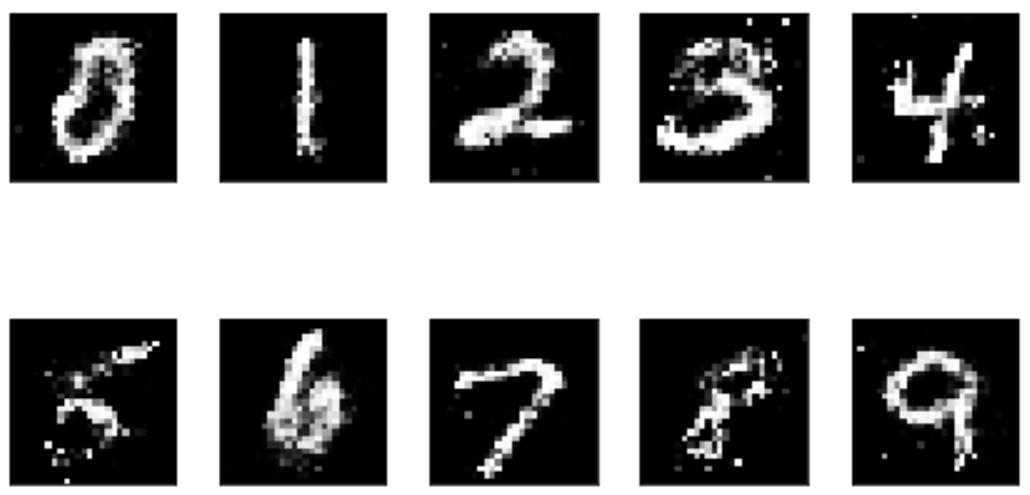
\includegraphics[width=7cm]{kapitel/2_stand_der_technik/img/cgan-notebook-ergebnisse.png}
	\caption{Ergebnisse Notebook \cite{cgan-tutorial-notebook}) }
\end{figure}

\subsection{LightCovidNet}
Das LightCovidNet \cite{inspiration-dc-gan-med} erlaubt die Erkennung von Krankheitsfällen in Lungen Röntgenscans.
Bei den Krankheitsbildern handelt es sich um COVID-19 und virale Lungenentzündungen.
Das Netz wurde dafür zum Teil auf synthetische COVID-19 Bilder trainiert, um einem Missverhältnis an Bildern für die Krankheiten in den Trainingsdaten entgegenzuwirken.
Das zur Generierung verwendete GAN erlaubt die Erzeugung von allen Krankheitstypen und auch Bildern von gesunden Lungen, wobei für die Arbeit nur die Generierung von COVID-19 Bildern von Interesse war.
\newline

Das dadurch entstandene GAN ist auch für diese Arbeit interessant, da es in der Lage ist, komplexe Formen mithilfe von relativ weniger Parameter zu generieren.
Die Parameteranzahl ist so gering, da in der Architektur hauptsächlich Convolutional(-Transpose) statt Dense-Layern eingesetzt werden.

\begin{figure}[H]
	\centering
	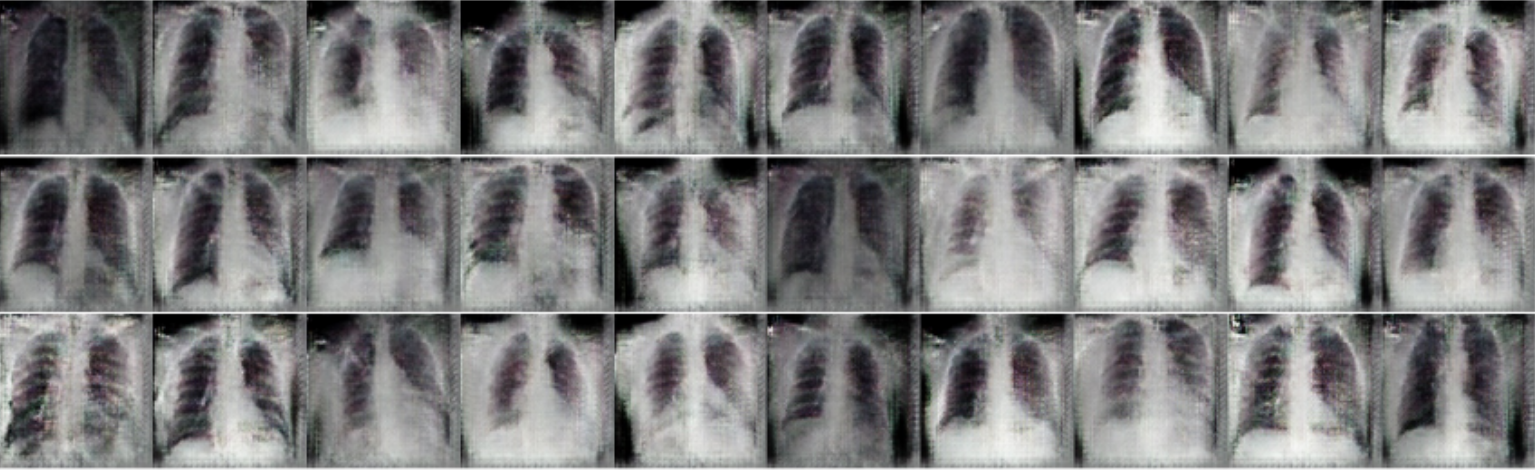
\includegraphics[width=9cm]{kapitel/2_stand_der_technik/img/light-covid-net-ergebnisse.png}
	\caption{Ergebnisse GAN aus LightCovidNet \cite{inspiration-dc-gan-med}}
\end{figure}


\begin{comment}
	
\paragraph{Links}
\begin{itemize}
	\item Inception Score zum Rating von erzeugten Bildern (Salimans et al. 2016)
	\item Frechet Inception Distance (Heusel et al. 2017)
	\item stackoverflow \url{https://stackoverflow.com/questions/46386948/adjusting-gan-hyperparameters}
	\item \url{https://openreview.net/pdf?id=rkGG6s0qKQ}
	\item \url{https://arxiv.org/pdf/1511.06434.pdf%C3%AF%C2%BC%E2%80%B0}
	\item Forget the Learning Rate, Decay Loss \url{https://arxiv.org/ftp/arxiv/papers/1905/1905.00094.pdf}
	\item beste learningRate/Dropout/BatchSize/NumberOfNeuronsInDenseLayer mit evolutionären neuronalen netz für mnist 
	\item zum orientieren ?? \cite{gan-conditional}
\end{itemize}


\end{comment}